

\documentclass[conference]{IEEEtran}


\ifCLASSINFOpdf
\else

\fi

\hyphenation{op-tical net-works semi-conduc-tor}

\usepackage{graphicx}
\usepackage{listings}
\usepackage[T1]{fontenc}
\usepackage{tikz}
\usetikzlibrary{arrows,calc,positioning}
\tikzstyle{intt}=[draw,text centered,minimum size=6em,text width=5.25cm,text height=0.34cm]
\tikzstyle{intl}=[draw,text centered,minimum size=2em,text width=2.75cm,text height=0.34cm]
\tikzstyle{int}=[draw,minimum size=2.5em,text centered,text width=3.5cm]
\tikzstyle{intg}=[draw,minimum size=3em,text centered,text width=6.cm]
\tikzstyle{sum}=[draw,shape=circle,inner sep=2pt,text centered,node distance=3.5cm]
\tikzstyle{summ}=[drawshape=circle,inner sep=4pt,text centered,node distance=3.cm]

\begin{document}
\title{Algorithms for Optimization of Big Data \\ Final Exam Report \\ }

\author{\IEEEauthorblockN{Malav Vora \\ 1401062}}
\maketitle

\begin{abstract}
Abstract In the given problem, we are given a big data of various details about many candidates. Based on this data, we apply big data algorithms and suggest a career path for the candidate based on his profile and skillset he possesses. 

\end{abstract}

\IEEEpeerreviewmaketitle



\section{Task - 1: Cleaning of data}

The given data is corrupted with some unicode values in it which are required to be removed/replaced with proper replacement. So, first we need to detect the unicodes by reading complete files and then replace it with proper content such that it is easier for us to read data when we use it for algorithms. First of all we read whole file and detect where the unicodes are as they start with ‘\u’. Whenever a unicode is detected, depending on what the unicode represents, the python code replaces it with its equivalent ASCII code so that is becomes easier for us to read it. This goes on till the end of file and then we have a data that is cleaned and completely in ASCII characters. Then this data is written in the file and algorithm are applied on it. 

\section{Task – 2 : Structuring of data}
To structure the clean data, it is converted to .csv from .txt file because it data in a .csv file is more structured and processing is easily possible in it than a .txt file. So, using json library of python, I load the whole file and seperate its content according to the fields provided like CandidateID, Company, job-Description, etc. This helps us get all the details of a candidate in a single column. This also stores all the data in python dictionary because of the format of given data. The algorithm for it is as follows:

\lstset{basicstyle=\small,style=myCustomMatlabStyle}

\begin{lstlisting}
# loads .txt file using json to read
with open("Automation Test Engineer
    .txt", "rb") as fin:
    content = json.load(fin)

# dumps content of .txt file using json 
# in the new file
with open("Automation Test Engineer json
    .txt", "wb") as fout:
    json.dump(content, fout, indent=1)

# load data of new json file using in 
# dictionary x
with open("Automation Test Engineer json
    .txt", "rb") as fin:
	x = json.load(fin)
	
f = csv.writer(open("filename.csv", "wb+"))

# Write CSV Header
f.writerow(["CandidateID", "Company",
            "Job-Description", "Job Title",
            "Job-Duration",  "Skills",
            "Additional-Info", "Location",
            "Institute", "School-Duration",
            "Qualification", "Resume-Summary"])

for x in x:
    f.writerow([x["CandidateID"],
                x["Work-Experience"]["Company"],
                x["Work-Experience"]["Job-Description"],
                x["Work-Experience"]["Job Title"],
                x["Work-Experience"]["Job-Duration"],
                x["Skills"],
                x["Additional-Info"],
                x["Location"],
                x["Education"]["Institute"],
                x["Education"]["School-Duration"],
                x["Education"]["Qualification"],
                x["Resume-Summary"]])

\end{lstlisting}

\section{Module 1: Read user's profile and suggest a career path - based on his skill set}
To suggest the candidate about his career path, we use the concept of nearest neighbours where more the common skills between candidates, nearer are the neighbours and hence more is their probability of having same career path. This methodology is also known as collaborative filtering which is used for recommending a user based on rating or reviews of other users. 

Now that we have organised data with us, we need to suggest a career path for a candidate. As the candidate logs in, we have his CandidateID and all of his details. We need to provide our suggestions based on the skills a candidate possesses. So, I take our candidate for whom we are suggesting a career path and all the other candidates with same profile(i.e. Automation Test Engineer, Computer Systems Manager, Customer Support Administrator, etc.) and check for the common skills between them. Then a list is created which has the candidates who have one or more skills common with the logged in candidate. Also this list is sorted such that other candidates having highest number of common skillset is first because it implies that both of them have more common  skills and so there is higher probability that the current candidate will follow his career path. Once we get the candidates whose path the current candidate is supposed to follow, we then take job detail of those candidates and suggest it to our candidate.
The module that gives similarities between the skillset of a candidate and other candidates is given below. It returns a list of his skillset with another candidate.

\begin{lstlisting}
	
def candSimilarity(candidate1, candidate2):
"""Computes the similarity between two 
candidates and their skills. Both 
candidate1 and candidate2 are
dictionaries. Candidate1 is the candidate 
whom we are suggesting career path and 
candidate2 will be all other candidates
having same title"""
  similarity = []
  for skill in candidate1:
    if skill in candidate2:
	  similarity.append(candidate1[skill]) 
  return similarity

\end{lstlisting}

This method gives the closest candidates i.e candidates having most common skillset with the candidate. It is a 2-dimensional list that has list of skills in common with every other candidate. 

\begin{lstlisting}

def closestCandidates(candidate1,candidates):
"""creates a sorted list of users based 
on skills to username"""
 similarity = []
 for candidate in candidates:
   if candidate != candidates:
    similarity = candSimilarity(candidate1,
                                candidate)
    similarity.append(similarity, candidate1)
    # sort based on distance -- closest first
   similarity.sort()
 return similarity
    
\end{lstlisting}

The method that helps a candidate find relatable career path is given below. It first checks the nearest neighbours i.e. candidates having most common skillset. Then using that it suggests the career path to the candidate depending on what other candidates have had already but this candidate hasn't. 
\begin{lstlisting}

def suggestCareerPathSkillset(candidate, 
                              candidates):
"""Give list of suggestions"""
# first find nearest neighbor
 closest = closestCandidates(candidate,
                             candidates)
 suggestions = []
 closeCandPath = candidates[jobTitle]
 candidateJob = candidate[jobTitle]
 for jobTitle in closeCandPath:
  if not jobTitle in candidate:
   suggestions.append(job-title,
                      closeCandPath[jobTitle])
 return sorted(suggestions, 
               skillset: skillset[1])

\end{lstlisting}

  \begin{figure}[!htb]
    \centering
    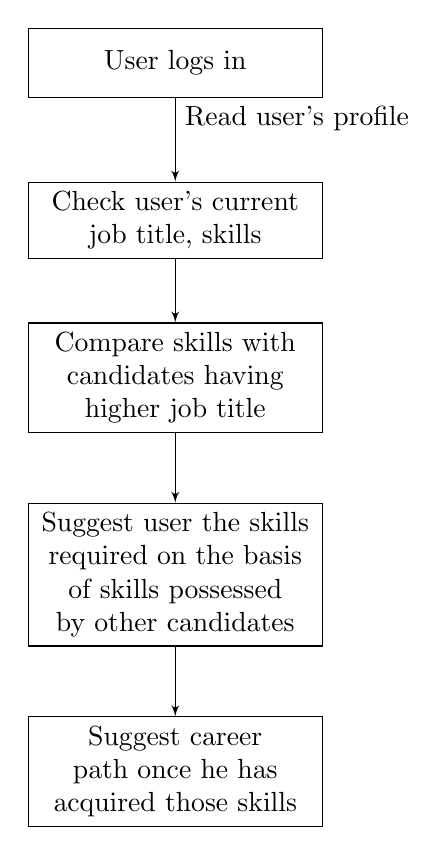
\begin{tikzpicture}[
      >=latex',
      auto
    ]
      \node [int] (kp)  {User logs in};
      \node [int] (kp1) [node distance=2cm,below of=kp] {Check user's current job title, skills};
	  \node [int] (kp2) [node distance=2cm,below of=kp1] {Compare skills with candidates having higher job title };

      \node [int]  (kp3) [node distance=2.5cm, below of=kp2] {Suggest user the skills required on the basis of skills possessed by other candidates};
      \node [int]  (kp4)[node distance=2.5cm, below of=kp3] {Suggest career path once he has acquired those skills};

      \draw[->] (kp) -> (kp1) node[right,pos=0.25] {Read user's profile};
      \draw[->] (kp1) -> (kp2);
      \draw[->] (kp2) -> (kp3);
      \draw[->] (kp3) -> (kp4);
    \end{tikzpicture}
    \caption{Flowchart of how user will be suggested his career path}
    \label{fig:datafusionindirectdirectfc}
  \end{figure}

\section{Module 2: User enters a career goal and suggest a career path - based on his career goal}

In this module we take a career goal as an input from user. Then we need to provide him a career path based on his goal. Here also we will have to use nearest neighbour and collaborative filtering. But here the nearest neighbours with whom we will compare will be only those candidates who have already achieved the career goal entered by user. We form a cluster of candidates who have achieved the goal and that is in their career path. Then using the concept of nearest neighbours, we find out candidates who have job profile and other additional information closest to the user. We sort them in order such that the nearest one is closest and so. From those candidates we select the path chosen by them from the user's current title to his goal. It is not necessary that each of those candidate will have same path. So we give the path in order that user needs to acquire minimum skill-set. In this way, user will then only be suggested career path based on his career goal. Fig. 2 is a flowchart explaining the flow from user entering his goal to the module suggesting him his career path.
\begin{figure}[!htb]
    \centering
    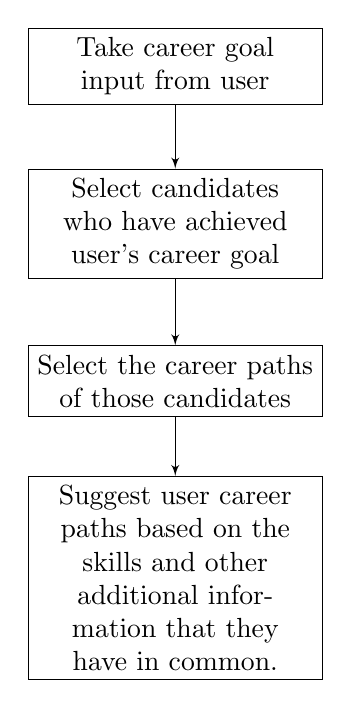
\begin{tikzpicture}[
      >=latex',
      auto
    ]
      \node [int] (kp)  {Take career goal input from user};
      \node [int] (kp1) [node distance=2cm,below of=kp] {Select candidates who have achieved user's career goal};
	  \node [int] (kp2) [node distance=2cm,below of=kp1] {Select the career paths of those candidates};

      \node [int]  (kp3) [node distance=2.5cm, below of=kp2] {Suggest user career paths based on the skills and other additional information that they have in common.};

      \draw[->] (kp) -> (kp1);
      \draw[->] (kp1) -> (kp2);
      \draw[->] (kp2) -> (kp3);
      \end{tikzpicture}
    \caption{Flowchart of how user will be suggested his career path on the basis of career goal}
    \label{fig:datafusionindirectdirectfc}
  \end{figure}


\section{Results}
Figure 3 and figure 4 are the results for Candidates 4 and 7 of Automation Test Engineer respectively.
\begin{figure}

  \includegraphics[width=\linewidth]{ss1.png}
  \caption{Career Path for Candidate 4 of Automation Test Engineer}
    
  \includegraphics[width=\linewidth]{ss2.png}
  \caption{Career Path for Candidate 7 of Automation Test Engineer}

\end{figure}
\section{Conclusion}

I was able to clean the data and fetch ASCII data such that processing is possible on that data. Then I applied  collaborative filtering algorithm for designing first module. I also tried to design second module but there were issues of reading other fields that had descriptive responses.   

\begin{thebibliography}{9}
\bibitem{latexcompanion} 
JohnS. Breese, David Heckerman and Carl Kadie . 
\textit{Empirical Analysis of  Predictive Algorithms for Collaborative Filtering}. 
Microsoft Research Redmond, WA 98052-6399  

\bibitem{latexcompanion} 
Ron Zacharski
\textit{A Programmer’s Guide to Data Mining: The Ancient Art of the Numerati}. 
 
\bibitem{latexcompanion} 
Badrul Sarwar, George Karypis, Joseph Konstan, and John Riedl
\textit{Item-Based Collaborative Filtering Recommendation Algorithms}. 
GroupLens Research Group/Army HPC Research Center, Department of Computer Science and Engineering, University of Minnesota, Minneapolis, MN 55455

\bibitem{Python Documents} 
Python Documents,
\\\texttt{https://docs.python.org/3/library/json.html}

\bibitem{Python Documents} 
Stackoverflow,
\\\texttt{http://stackoverflow.com/questions\\/3368969/find-string-between-two-substrings}

\bibitem{Python Documents} 
json,
\\\texttt{http://stackoverflow.com/questions\\/20901018/converting-string-file-into-json-format\\-file}

\bibitem{Python Documents} 
Substring,
\\\texttt{http://stackoverflow.com/questions\\/12572362/get-a-string-after-a-specific-substring}

\bibitem{Python Documents} 
Unicode to ASCII,
\\\texttt{http://stackoverflow.com/questions\\/175240/how-do-i-convert-a-files-format-from-unicode\\-to-ascii-using-python}

\end{thebibliography}


\end{document}



